\chapter{Preference Change}\label{ch:7}

Preferences play a central role in theories of decision making
as part of the mechanism underlying intentional behavior and rational choice:
they show up in economic models of rational 
agency \cite{MasColell95,Sen17},
as well as in formal models of artificial agents 
supposed to interact with the world and each 
other \cite{BoutilierBDHP04,DomshlakHKP11,RossiVW11,PigozziTV16}.
Since such interactions take place in dynamic environments, 
it can be expected that preferences change in response to new developments.

In this chapter we are interested in preference change 
occurring when new preference information,
denoted by $\o$, becomes available and has to be taken at face value, 
thereby prompting a change in prior preference information, denoted by $\p$.
The change, we require, should preserve as much useful information from $\p$
as can be afforded.

We believe that preference change thus described is a pervasive phenomenon, 
arising in many contexts straddling the realms of both human and artificial agency.
Thus, there is a distinguished tradition in economics and philosophy
puzzling over examples of conflict between an agent's subjective preference
(what we call here the initial, or prior preference $\p$) 
and a second-order preference,
often standing for a commitment or moral rule 
(what we call here the new preference information $\o$):
the need to reconcile such a conflict is widely acknowledged, but in the absence
of a concrete mechanism for doing so its presence is more often than not 
simply signaled as a problem that besets real life agents.
% \cite{Harsanyi55,Jeffrey74,Sen77,Frankfurt88,Nozick94}.

One example of the phenomenon that leads to preference revision
occurs in the philosopher Harry Frankfurt's discussion on  
\emph{second-order volitions}, which are desires about desires.
According to Frankfurt, an agent's second-order volition with respect 
to a desire $D$ is a desire that $D$ be the agent's will, 
i.e., that $D$ determines the agent's actions:
\begin{quote}
	Besides wanting and choosing and being moved to do this or that, 
	[people] may also want to have (or not to have) certain desires and motives. 
	They are capable of wanting to be different, 
	in their preferences and purposes, from what they are.
	\cite{Frankfurt88}
\end{quote}

The existence of second-order volitions is taken by Frankfurt 
to be a hallmark of personhood:

\begin{quote}
	\dots it is having second-order volitions [\dots] 
	that I regard as essential to being a person.
	\cite{Frankfurt88}
\end{quote}

Frankfurt does not mention preferences explicitly but, 
since in standard models of rational agency
preferences are taken to be part of what determines action, 
we can imagine that his point applies to preferences as well as desires.
Preferences do appear in subsequent discussions, for instance
in Robert Nozick's account of the same phenomenon:

\begin{quote}
	A person lacks rational integration when [they] prefer some alternative $x$ 
	to another alternative $y$, yet [they] prefer that [they] 
	did not have this preference, 
	that is, when [they] also prefer not preferring $x$ to $y$ 
	to preferring $x$ to $y$. 
	When such a second-order preference conflicts with a first-order one, 
	it is an open question which of these preferences should be changed. 
	What is clear is that they do not hang together well, 
	and a rational person would prefer that this not (continue to) be the case.
	\cite{Nozick94}
\end{quote}

Nozick's formulation brings us closer to the framework 
we will be using in this chapter, of preference orders battling it out.
If we assimilate his second order preferences to Frankfurt's second 
order volitions, then we have the same problem of a mismatch, 
or `lack of integration',
between the agent's preferences.
Nozick confines himself to just labeling the problem and does not tell 
us how to solve it, but we are led to understand that it is,
notwithstanding, a problem.
The same issue arises in economist John C. Harsanyi's
distinction between an individual's 
\emph{social welfare function} and their \emph{personal utility function},
two notions that refer to two distinct types of preferences:

\begin{quote}
	\dots the former [type of preference] 
	must express what this individual prefers 
	(or rather, would prefer) on the basis of 
	impersonal social considerations alone, 
	and the latter must express what he actually prefers, 
	whether on the basis of his personal 
	interests or on any other basis. 
	The former may be called his `ethical' preferences, 
	the latter his `subjective' preferences.
	\cite{Harsanyi55}
\end{quote}

In Harsanyi's phrasing, the problem is, as for Nozick, one of conflict
between preferences: humans are the kind of beings that can 
entertain two types of preferences at the same time,
and sometimes these preferences are not perfectly aligned.
At the same time, Harsanyi seems to suggest, the ethical preferences
(which we may assimilate with Frankfurt's second order desires
and Nozick's second order preferences)
enjoy a certain type of prestige over the other,
such that in a perfect world the subjective preferences 
would coincide with the ethical preferences,
but in the imperfect world we live in the two are sometimes 
at odds with one another.
That this is eminently possible is, of course, 
an old adage, and the phenomenon is sometimes called \emph{akrasia}
from the Greek term for lack of will.
A classical example of akrasia occurs with habits that people
want to get rid of, such as smoking: 
an agent smokes, which according to the revealed preference paradigm
we have been espousing in the previous chapters,
can be taken to indicate a preference of smoking over non-smoking;
but at the same time, the agent might want to quit,
i.e., to have the opposite preference.
In the context of decision theory, this problem shows up in the form 
of Richard C. Jeffrey's Akrates, 
who would rather be abstinent than smoke:

\begin{quote}
	\dots although Akrates cannot simply choose to prefer abstinence 
	on this occasion---and that, after all, is why his preference 
	for preferring abstinence is (uneasily) compatible with his 
	preference for smoking---he can undertake a project of modifying 
	his preferences over time, so that one day he may regularly prefer 
	abstinence, just as now he regularly prefers smoking. 
	The steps toward this desired end may involve hypnosis, 
	reading medical textbooks, discussing matters with like-minded friends, 
	or whatever. But in accounting for Akrates's undertaking of these 
	activities it seems natural to cite his preference for preferring 
	abstinence, just as in accounting for his activities as he flings 
	drawers open and searches through pockets of suits, 
	one may cite his preference for smoking\dots 
	\cite{Jeffrey74}
\end{quote}

Jeffrey, just like Frankfurt, Nozick and Harsanyi,
is interested here only in pointing out the basic fact 
that Akrates can prefer smoking to abstinence, 
while wishing he had the opposite preference.
Jeffrey assumes that Akrates' problem will be solved 
if Akrates can only get himself, by whatever means necessary,
to change his disposition such that he comes to 
prefers abstinence to smoking.
The challenge Akrates is facing is that he needs to
make sure that his priorities 
are aligned with the preferences specific to a respected source.
The same challenge can occur in technological applications, 
from updating CP-nets~\cite{CadilhacALB15}
to changing the order in which search results 
are displayed on a page in response to user provided specifications.
Similar topics are emerging in the discussion 
on ethical decision making for artificial agents \cite{RossiM19}.
Thus, far from being an issue of narrow interest, 
the problem of changing preferences and 
resolving conflicts along the way is an important 
component of rational agency.

Whether it is the internal conflict between 
an agent's private leanings and the better angels of its nature,
or a content provider wanting to tailor its products 
for a better user experience, 
many cases of preference change involve a conflict
between two types of preferences, one of which is 
perceived as having priority over the other:
we will call this type of change 
\emph{preference revision}, due to its similarity 
with revision as presented in Section \ref{sec:3-revision}.

Up to this point we have been arguing that 
cases of preference revision can arise in several contexts, 
but have not seen any actual mechanism for handling them.
What is Akrates to do?
Indeed, if there are only two alternatives 
to work with,
e.g., smoking and abstinence, 
then it is difficult to see what more can be said,
at the formal level, other than that smoking and abstinence 
should be swapped in Akrates' preference order.
To see that there is more at stake here, 
we must look at an example with more than two alternatives.

\begin{figure}\centering
	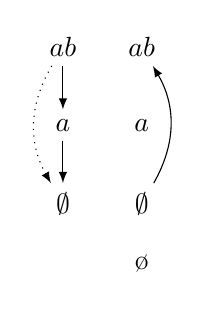
\begin{tikzpicture}
	\node at (0,-0.75){$\p$};
	\node at (0,2)(1){$ab$};
	\node at (0,1)(2){$a$};
	\node at (0,0)(3){$\emptyset$};
	\path[-latex](1)edge(2)(2)edge(3)(1)edge[bend right,dotted](3);
	
	\node at (1,-0.75){$\o$};
	\node at (1,2)(1){$ab$};
	\node at (1,1)(2){$a$};
	\node at (1,0)(3){$\emptyset$};
	\path[-latex](3)edge[bend right](1);
	
	\end{tikzpicture}		
	\caption{
		Preference order $\p$ has to be revised by
		preference $\o$.
		A direct comparison ranking $i$ better than $j$ is
		depicted by a solid arrow from $i$ to $j$, 
		with comparisons inferred by transitivity depicted by dotted arrows.
		To distinguish these types of preference orders 
		from the preference orders used to model belief change operators 
		in assignments, we draw the better elements on top here.
		}
	\label{fig:7-pref-change-3-alternatives}
\end{figure}

\begin{xmpl}{}{7-pref-change-3-alternatives}
	Consider the scenario from Example \ref{ex:1-pref-change-motivation},
	where a doctor is considering treatments for a novel disease. The 
	doctor has two drugs, $a$ and $b$, that can be prescribed alone 
	or in combination with each other. For the purposes of this illustration,
	let us assume the doctor is considering three alternatives:
	either to administer $a$ and $b$ together, denoted by the interpretation $ab$,
	or $a$ alone, denoted by the interpretation $a$,
	or nothing, denoted by $\emptyset$.

	The doctor's initial assessment is that 
	$a$ and $b$ together work better than $a$ alone, which 
	by itself is better than doing nothing.
	This ranking constitutes a preference order, 
	and by virtue of transitivity we can conclude 
	that $a$ and $b$ together are better
	than administering nothing.
	We can write the doctor's preferences as the set 
	$\p=\{(ab,a),(a,\emptyset),(ab,\emptyset)\}$
	of comparisons the doctor bases its assessment on.
	The comparison $(ab,a)$, for instance, is to be read 
	that $ab$ is strictly better than $a$.
	Of the comparisons in $\p$, we may assume that $(ab,a)$ and $(a,\emptyset)$
	are established by the doctor directly,
	while $(ab,\emptyset)$ is inferred by transitivity from the other two.
	The preference order $\p$ is depicted in Figure \ref{fig:7-pref-change-3-alternatives}.

	Afer a while, the doctor becomes convinced that $\emptyset$ is better than $ab$,
	and hence has to modify its initial assessment $\p$ accordingly.
	We can represent the new information as a preference order $\o$ in its own right.
	The preference order $\o$ consists of the comparison $(\emptyset,ab)$,
	i.e., $\o=\{(\emptyset, ab)\}$, 
	and is likewise depicted in Figure \ref{fig:7-pref-change-3-alternatives}.
	Note that simply adding $\o$ to $\p$
	leads to a cycle between the three alternatives,
	i.e., the transitive closure of $\p\cup\o$ implies that 
	$ab$ is strictly better than itself.
	Since the doctor is committed to accepting $\o$,
	then they will have to give up something from $\p$ in order to maintain 
	consistency. 	
\end{xmpl}

Example \ref{fig:7-pref-change-3-alternatives} is not a case of akrasia,
but illustrates the problem just as well:
if new preference information contradicts an existing preference,
in the sense that it leads to a preference cycle,
then some of the comparisons involved in the cycle have to be given up.
The challenge for Akrates, then, is that even after fitting 
the second order preference into his schedule,
he still needs to figure out what the rest of his preference order
looks like. In other words, Akrates has a decision problem on his hands:
since there is no unique way, on logical grounds alone, 
of breaking a preference cycle, some extra information needs to be brought in.
What should this extra information concern?

Based on our experience so far, 
we should expect the answer to be preferences:
indeed, preferences on preferences themselves.
This strategy, which we will be pursuing in the 
rest of this chapter,
has already been anticipated by Amartya Sen:

\begin{quote}
	...we need to consider rankings of preference rankings to express our moral judgments.
	\cite{Sen77}
\end{quote}

We want to pick up Sen's suggestion and 
suggest that preferences over the basic building
blocks of a preference order, 
i.e., the comparisons it is made of, 
offer a way of understanding preference revision.

\begin{figure}\centering
	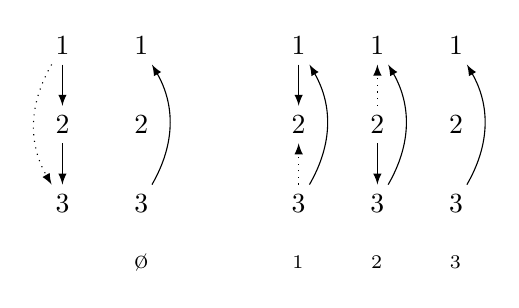
\begin{tikzpicture}
	\node at (0,-0.75){$\p$};
	\node at (0,2)(1){$1$};
	\node at (0,1)(2){$2$};
	\node at (0,0)(3){$3$};
	\path[-latex](1)edge(2)(2)edge(3)(1)edge[bend right,dotted](3);
	
	\node at (1,-0.75){$\o$};
	\node at (1,2)(1){$1$};
	\node at (1,1)(2){$2$};
	\node at (1,0)(3){$3$};
	\path[-latex](3)edge[bend right](1);
	
	\node at (3,-0.75){$\p_1$};
	\node at (3,2)(1){$1$};
	\node at (3,1)(2){$2$};
	\node at (3,0)(3){$3$};
	\path[-latex](3)edge[bend right](1)(1)edge(2)(3)edge[dotted](2);
	
	\node at (4,-0.75){$\p_2$};
	\node at (4,2)(1){$1$};
	\node at (4,1)(2){$2$};
	\node at (4,0)(3){$3$};
	\path[-latex](3)edge[bend right](1)(2)edge(3)(2)edge[dotted](1);
	
	\node at (5,-0.75){$\p_3$};
	\node at (5,2)(1){$1$};
	\node at (5,1)(2){$2$};
	\node at (5,0)(3){$3$};
	\path[-latex](3)edge[bend right](1);
	\end{tikzpicture}		
	\caption{
		Revising preference order $\p$ by $\o$: 
		simply adding $\o$ to $\p$ leads to a cycle,
		so if $\o$ is accepted then a choice needs 
		to be made regarding which of the initial comparisons of $\p$ to keep;
		potential candidates for the revised order are $\p_1$, $\p_2$ or $\p_3$.
		A direct comparison ranking $i$ better than $j$ is	depicted by a solid arrow from $i$ to $j$, 
		with comparisons inferred by transitivity depicted by dotted arrows.
		}
	\label{fig:7-pref-change-3-alternatives-ctd}
\end{figure}

\begin{xmpl}{}{7-pref-change-3-alternatives-ctd}
	We revisit the scenarion in Example \ref{ex:7-pref-change-3-alternatives},
	with a doctor revising their preferences over three treatment options:
	$ab$, $a$ and $\emptyset$.
	To further simplify the problem, we denote the alternatives by 
	integers, such that $1$ stands for $ab$, $2$ stands for $a$ and $3$ stands for $\emptyset$. 
	The initial preference $\p$ is such that,
	as a result of direct comparison, 
	alternative $1$ is ranked better than $2$ 
	and $2$ is ranked better than $3$;
	by virtue of transitivity, it is also inferred that 
	$1$ is considered better than $3$.
	We want to revise $\p$ by a preference $\o$, 
	according to which $3$ is better than $1$. 
	Both preference orders $\p$ and $\o$ are depicted in 
	Figure \ref{fig:7-pref-change-3-alternatives-ctd}.
	%	this means that $\p$ has to be modified to incorporate the comparisons contained in $\o$,
	%	but without giving up more information than strictly necessary.

	The simplest solution is to add $\o$ to $\p$ 
	(i.e., include the comparisons contained in both),
	but the transitivity requirement leads to a cycle between $1$, $2$ and $3$, 
	%	and thus the result fails to be a preference order.
	which we would like to avoid.
	We are thus in a situation where $\p$ and $\o$ cannot be jointly accepted,
	but since $\o$, we stipulate, must be accepted,
	something must be given up from $\p$ (though,
	we ask, no more than strictly necessary). How is the decision to be made?
	We suggest that an implicit preference over the comparisons of 
	$\p$ that were explicitly provided
	can provide an answer: if the comparison of $1$-vs-$2$ 
	(the edge from $1$ to $2$ in Figure \ref{fig:7-pref-change-3-alternatives-ctd})
	is preferred to the one of $2$-vs-$3$ then the result is $\p_1$, which
	holds on to $1$-vs-$2$ from $\p$ and together with $\o$ infers, by transitivity, 
	that $3$ is better than $2$;
	alternatively, a preference for $2$-vs-$3$ over $1$-vs-$2$
	leads to $\p_2$ as the result, while indifference between the two comparisons
	means that both are given up, resulting in $\p_3$.
	Thus, preference over comparisons in $\p$ translates as choice over how to go about revising $\p$.
	Interestingly, we may also reason in the opposite direction:
	observing choice behavior across different instances of revision allows us to infer preferences 
	over comparisons in $\p$, e.g., revising to $\p_1$, rather than to $\p_2$ or $\p_3$,
	can be rationalized as saying that the comparison of $1$-vs-$2$
	is considered better than $2$-vs-$3$.
\end{xmpl}

Our aim in this chapter is to formalize the type of 
reasoning illustrated in Example \ref{ex:7-pref-change-3-alternatives-ctd}
by rationalizing preference change as a type of choice function 
on what we will call the \emph{direct comparisons of $\p$},
i.e., the explicit preferences assumed to be given in $\p$.
Since a conflict between $\p$ and $\o$ forces some of the direct comparisons of $\p$
to be renounced, additional information in the form of a preference order over the direct comparisons
of $\p$ will serve as guide to the choice function.
%Revising an initial preference $\p$ by new preference information $\o$,
%especially if $\p$ and $\o$ are conflicting,
%opens up a range of options, as Example \ref{ex:preferences-3-items} illustrates.
Our purpose, in this, is not to legislate on what is the right choice to make;
rather, it is to make sure that whatever the choice is, it is made in a coherent way.
To this end, we present a set of rationality postulates 
to capture conditions under which the preference order on direct comparisons of $\p$ 
exists and has desired properties.
Thus, the significance of our approach lies in laying bare the theoretical requirements
and basic assumptions for mechanisms intended to revise preferences.

The postulates we put forward bear a distinct resemblance to the AGM postulates 
employed for belief revision
\cite{AlchourronGM85,KatsunoM92,Hansson17,FermeH18}:
given that changing one's mind involves choosing some parts 
of a belief to keep and some to remove,
this is no coincidence. 
Indeed, the two problems are similar, 
though the structural particularities of preferences
(in particular, the requirement that they are transitive) 
mean that transfer of insights from belief revision 
to preference revision is by no means straightforward.

%In this paper, we model preference change arising out of an interaction between two elements:
%the first is an initial preference ranking, typically denoted by $\p$,
%which encodes a pre-existing attitude;
%the second element is new preference information $\o$ signaling input from an authoritative source,
%which may come into conflict with the information in $\p$.
%The assumption is that $\o$ has priority,
%but that $\p$ contains useful information which should not be discarded unless absolutely necessary.
%Thus, the presence of $\o$ triggers a change in $\p$, 
%the latter having to be modified in an efficient way such that it accommodates $\o$:
%the end goal is to bring $\p$ in line with $\o$, without having to give up more of $\p$ than is needed.
%Formally, this is performed by a change operator $\en$,
%the result of which is a new preference order, typically denoted by $\p\en\o$,
%which fully incorporates $\o$ while preserving as much as possible from the pre-existing order $\p$. 


% The rest of the paper contains our contributions, summarized as follows. 
% In Section \ref{sec:preliminaries}
% we introduce basic notation.
% In Section \ref{sec:semantics} we provide a constructive way of revising a preference order,
% based on rankings of the direct comparisons.
% In Section \ref{sec:postulates} we provide a set of intuitive postulates 
% and we show that they characterize the procedure described in Section \ref{sec:semantics}.
% Section \ref{sec:concrete-operator} discusses concrete preference revision operators,
% and Section \ref{sec:conclusion} offers concluding remarks.














\section{Strict partial orders}\label{sec:7-spos}
We assume a finite set $V$ of items, 
standing for the objects an agent can have preferences over.
In keeping with the pattern established so far, 
a preference order is construed as a transitive binary relation on $V$, 
though in a break with standard practice 
the preferences that undergo change are denoted here by 
$\p$ and $\o$, rather than $\le$, to avoid confusion with the 
preferences used to model a belief change operator. 
Preferences that undergo revision are expected to
satisfy, for any $x$, $x_1$ and $x_2$ in $V$,
some combination of the following properties:
\begin{description}
	\item[($\oop{2}$)] If $x_1\le x_2$ and $x_2\le x_3$, then $x_1\le x_3$. \hfill(transitivity)
	\item[($\oop{3}$)] If $x_1\neq x_2$, 
		then $x_1 \le x_{2}$ or $x_{2} \le x_{1}$. \hfill(totality)
	\item[($\oop{4}$)] $x\not\le x$. \hfill(irreflexivity)
\end{description}

Properties $\oop{2-4}$ accompany the properties provided in Section \ref{sec:2-preferences},
which is why $\oop{1}$ is absent from the current lineup.
If $\p$ is a binary relation on a set $V$ of items,
then $\p$ is a \emph{strict partial order (spo) on $V$}
if $\p$ satisfies properties $\oop{2}$ and $\oop{4}$,
i.e., if $\p$ is transitive and irreflexive.
We write $\SPO_V$ for the set of strict partial orders on $V$.
If $\p$ is an spo on a set $V$ of items, 
then $\p$ is a \emph{strict linear order on $X$} if $\p$
also satisfies property $\oop{3}$,
i.e., if $\p$ is total, in addition to being transitive and irreflexive.
A \emph{chain on $V$} is a strict linear order on a subset of $V$.
We write $\CHN_V$ for the set of chains on $V$.
% Note that if $\le$ is a linear order on $X'\subseteq X$, then 
% property $\oop{3}$ implies that $\le$ also satisfies property $\oop{1}$ on $X'$.

If $\p$ is an spo on a set of items $V$,
then a \emph{comparison $(i,j)$ of $\p$} 
is an element $(i,j)\in\p$, for some items $i,j\in V$,
interpreted as saying that, in the context of $\p$, 
$i$ is considered strictly better than $j$.
To simplify notation, 
we sometimes also refer to comparisons with the letter $c$.
We often have to consider the union $\p_1\cup\p_2$ of two spos,
which is not guaranteed to be an spo, 
since transitivity is not preserved under unions.
If this is the case, we typically have to 
substitute $\p_1\cup\p_2$ for its 
\emph{transitive closure}, denoted by $(\p_1\cup\p_2)^+$.
%is the relation obtained 
%by adding to $\rho$ all elements $(i,j)$ such that there exist items $k_1$, \dots, $k$ in $V$
%such that $i=k_1$, $j=k$ and $(k_1,k_2)$, $(k_2,k_3)$, \dots, $(k_{m{-}1},k_m)$ are in $\rho$. 
% Mostly for technical reasons we will ignore comparisons $(i,i)$, for $i\in V$, whenever they occur.
%i.e.,
%we stipulate that $(i,i)=\emptyset$.
% We will assume that the initial preference order $\p$ 
% is a linear order on a subset of $V$,
% with $\CHN_V$ being the set of all such linear orders,
% while the new preference order $\o$ is a strict partial order (spo) on $V$,
% with $\SPO_V$ being the set of all such spos.
% Additionally, $\TPRE_{V\times V}$ and $\CHN_{V\times V}$ are the sets 
% of total preorders and linear orders, respectively, over subsets of $V\times V$.
%Note that a preference ranking in $\CHN_V$ is not required to rank all items in $V$.
Since preferences are required to be transitive, we write a sequence of comparisons
$\{(1,2),(2,3)\dots,(m{-}1,m)\}^+$ as $(1,\dots, m)$.

%We will find it useful to distinguish between the comparisons in a preference order.
If $\p = (i_1,\dots, i_m)$ is a chain on $V$,
a \emph{direct comparison of $\p$} is a comparison 
$(i_k,i_{k+1})\in\p$,
i.e., a comparison between $i_k$ and its direct successor in $\p$,
with $\dir_\p$ being the set of direct comparisons of $\p$.
The assumption is that direct comparisons are the result of explicit information, 
and are basic in the sense that they cannot 
be inferred by transitivity using other comparisons in $\p$.
Given preference orders $\p\in\CHN_V$ and $\o\in\SPO_V$, we want to carve out the
possible options for the revision of $\p$ by $\o$.
For this we use the set $\upper{\o}_\p$ of \emph{$\p$-completions of $\o$}, defined as:
$$
\upper{\o}_\p = \{(\o\cup\d)^+\in\SPO_V\mid\d\subseteq\dir_\p\}.
$$
The intuition is that a $\p$-completion of $\o$ is a preference order
constructed from $\o$ using some, and only, direct comparisons in $\p$, i.e., information
originating exclusively from the two sources given as input.
We will expect that a preference revision operator selects one element of this set as
the revision result.
%More motivation on why this these are the results worth wanting is
%given in Section \ref{sec:postulates}.  
%Note, for now, that $\o\subseteq\o'$, for any $\o'\in\upper{\o}_\p$.

Though taking $(\p\cup\o)^+$ as the result of revising $\p$ by $\o$ is not, in general, feasible,
we still want to identify parts of $(\p\cup\o)^+$ that are uncontroversial.
To that end, the \emph{cycle-free part $\cycfree{\p}{\o}$ of $(\p\cup\o)^+$} is defined as:
$$
\cycfree{\p}{\o} = \{\drc{i}\in(\p\cup\o)^+\mid(\tightplus{i}{1},i)\notin(\p\cup\o)^+\},
$$
i.e., the set of comparisons of $(\p\cup\o)^+$ not involved in a cycle with the comparisons of $\o$.
The \emph{cyclic part $\cyc{\p}{\o}$ of $\p$ with respect to $\o$} is defined as:
$$
\cyc{\p}{\o} = \{\drc{i}\in\dir_\p\mid(\tightplus{i}{1},i)\in(\p\cup\o)^+\},
$$
i.e., the set of direct comparisons of $\p$ involved in a cycle with $\o$.

\begin{xmpl}{}{7-completions}
	For $\p$ and $\o$ as in Example \ref{ex:7-pref-change-3-alternatives-ctd}, 
	we have that $\dir_\p=\{(1,2),(2,3)\}$,
	while the $\p$-completions of $\o$ are 
	$\upper{\o}_\p=\{(3,1,2), (2,3,1), (3,1)\}$,
	i.e., the spos obtained by adding to $\o$ either of the elements of $\dir_\p$, or none
	(corresponding to $\p_1$, $\p_2$ and $\p_3$).
	The cyclic part of $\p$ with respect to $\o$ is 
	$\cyc{\p}{\o}=\dir_\p=\{(1,2),(2,3)\}$
	and
	the cycle-free part of $\p$ with respect to $\o$ is
	$\cycfree{\p}{\o}=\emptyset$.
\end{xmpl}


% For reasons of space we do not include here the model of propositional belief revision,
% though readers familiar with it will notice common themes and interesting departures.

















\section{A general method for revising preferences}\label{sec:7-semantics}
A \emph{preference revision operator $\en$}
is a function
$\en\colon\CHN_V\times\SPO_V\rightarrow\SPO_V$ 
taking a chain $\p$ and an spo $\o$ as input, 
and returning an spo $\p\en\o$ as output.
The choice of input and output can be motivated by a short nod to the 
material that is to come: since we will be rationalizing 
preference revision operators using preferences (i.e., preorders) on comparisons,
an spo as output reflects the fact that certain comparisons are 
considered equally good, and must be given up together. 
The unfortunate effect of this, of course, is that the input and output formats do not match,
which makes it impossible to iterate the revision operation.
That being said, the output could be tightened to a chain: provided that the preferences 
guiding revision are a linear order (i.e., there are no ties); this will be touched on 
at the end of Section \ref{sec:7-representation}.
Making both the input and output spos would be desirable, 
but intricacies of getting details right here means that this is best left for future work.

We start, then, by presenting a general procedure for revising preferences that, as advertised,
utilizes total preorders on the set $\dir_\p$ of direct comparisons of $\p$:
thus, a \emph{preference assignment $\as$} is a function 
$\as\colon\CHN_V\rightarrow\TPRE_{V\times V}$ mapping
every preference $\p\in\CHN_V$ to a 
total preorder $\le_\p$ on elements of $V\times V$, 
i.e., on pairwise comparisons on the items of $V$, 
of which we are interested only in the preorder on $\dir_\p$.
In typical AGM manner, a comparison $c_i\le_\p c_j$ 
in the context of a preorder $\le_\p$ on $\dir_\p$ means
that $c_i$ is \emph{better} than $c_j$.

If $\p\in\CHN_V$, $\o\in\SPO_V$ and $\le_\p$ is a total preorder on 	$\dir_\p$,
then, for $i\geq 1$, the \emph{$\le_\p$-level $i$ of $\dir_\p$}, denoted $\lvl_\le^i(\dir_\p)$,
contains the $i^\text{th}$ best elements of $\dir_\p$ according to $\le_\p$,
i.e., 
$\lvl^1_{\le_\p}(\dir_\p)=\min_{\le_\p}(\dir_\p)$,
$\lvl^{i+1}_{\le_\p}(\dir_\p)=\min_{\le_\p}(\dir_\p\setminus\bigcup_{1\leq j\leq i}\lvl^j_{\le_\p}(\dir_\p))$, etc.
%\begin{align*}
%\lvl_{\le_\p}^1(\p) &= \min_{\le_\p}(\dir_\p),\\
%\lvl_{\le_\p}^{i+1}(\p) &= \min(\dir_\p\setminus\lvl_{\le_\p}^i(\dir_\p)).
%\end{align*}
Note that the $\le_\p$-levels of $\dir_\p$ partition $\dir_\p$ and, since $\dir_\p$ is finite,
there exists a $j>0$ 
%after which there is nothing left to partition, i.e., 
such that $\lvl^i_{\le_\p}(\dir_\p)=\emptyset$, for all $i\ge j$.
%We then introduce 
The \emph{addition operator $\add^i_{\le_\p}(\o)$} is defined, 
for any $\o\in\SPO_V$ and $i\geq 0$, as follows:
\begin{align*}
\add_{\le_\p}^0(\o) &= (\o\cup\cycfree{\p}{\o})^+,\\
\add_{\le_\p}^i(\o) &= 
\begin{cases}
(\add^{i-1}_{\le_\p}(\o)\cup(\lvl_{\le_\p}^i(\dir_\p)\cap\cyc{\p}{\o}))^+,~\text{if in}~\SPO_V,\\
\add_{\le_\p}^{i-1}(\o),~\text{otherwise}.
\end{cases}
\end{align*}
\noindent
Intuitively, the addition operator starts by adding to $\o$ 
all the direct comparisons of $\p$ that are not involved in a cycle with it,
i.e., which are not under contention by the accrual of new preference information.
Then, at every further step $i>0$, the addition operator 
tries to add all comparisons on level $i$ of $\dir_\p$
that are involved in a cycle with $\o$:
if the resulting set of comparisons can be construed as a spo 
(by taking its transitive closure) the operation is successful, and the new comparisons are added;
if not, the addition operator does nothing.
Since the addition of new comparison follows the order $\le_\p$, this ensures
that better quality comparisons are considered before lower quality ones.

Note, this procedure guarantees that there are always \emph{some} comparisons in $\p\en\o$, i.e.,
$\o\subseteq\p\en\o$ regardless of anything else.
Note, also, that the number of non-empty levels in $\dir_\p$ is finite and
the addition operation eventually reaches a fixed point, i.e., there exists $j\ge 0$ such that
$\add^i_{\le_\p}(\o)=\add^j_{\le_\p}(\o)$, for any $i\ge j$.
We denote by $\add_{\le_\p}^\ast(\o)$ the fixed point of this operator and take it as the defining expression of
a preference revision operator: if $\as$ is a preference assignment,
then the \emph{$\as$-induced preference revision operator $\en^\as$} 
is defined, for any $\p\in\CHN_V$
and $\o\in\SPO_V$, as:
$$
	\p\en^\as\o\defeq\add^\ast_{\le_\p}(\o).
$$
Note that, by design, $\add^\ast_{\le_\p}(\o)\in\SPO_V$, i.e., the operator $\en$ is well defined.

\begin{figure}\centering
	\begin{tikzpicture}
	\node at (0,-1.5){$\p$};
	\node at (0,1.8)(1){$1$};
	\node at (0,0.9)(2){$2$};
	\node at (0,0)(3){$3$};
	\node at (0,-0.9)(4){$4$};
	\path[-latex](1)edge(2)(2)edge(3)(3)edge(4);
	\path[-latex,dotted](1)edge[bend right](3)(2)edge[bend right](4)(1)edge[bend right=40](4);
	
	\node at (1,-1.5){$\o$};
	\node at (1,1.8)(1){$1$};
	\node at (1,0.9)(2){$2$};
	\node at (1,0)(3){$3$};
	\node at (1,-0.9)(4){$4$};
	\path[-latex](3)edge[bend right](1);
	
	\node at (3,-1.5){$(\p\cup\o)^+$};
	\node at (3,1.8)(1){$1$};
	\node at (3,0.9)(2){$2$};
	\node at (3,0)(3){$3$};
	\node at (3,-0.9)(4){$4$};
	\path[-latex](1)edge(2)(2)edge(3)(3)edge(4)(3)edge[bend right](1);
	\path[-latex,dotted]
	(1)edge[bend right=60](3)(2)edge[bend right=50](4)
	(1)edge[bend right=70](4)(2)edge[bend left=30](1)
	(3)edge[bend left=30](2);
	
	\node at (5, -1.5){$\le_\p$};		
	\node at (5,-0.9){$(1,2)$};
	\node at (5,0){$(2,3)$, \sout{$(3,4)$}};
	\node at (6.5,-0.9){\tiny $\lvl^1_{\le_\p}(\p)$};
	\node at (6.5,0){\tiny $\lvl^2_{\le_\p}(\p)$};
	\end{tikzpicture}	
	\caption{
		Preference revision by adding direct comparisons from $\p$ to $\o$, using the preorder $\le_\p$.
		In $\le_\p$ lower means better; the comparison $(3,4)$ is ignored by the addition operator because it
		is not involved in a cycle with $\o$ (and is added at the beginning anyway).
	}
	\label{fig:7-preferences-4-items}
\end{figure}

\begin{xmpl}{}{7-preferences-4-items}
	For 
	%	$V=\{1,2,3,4\}$ and 
	$\p=(1,2,3,4)$, $\o=(3,1)$,
	we obtain that $\dir_\p=\{(1,2),(2,3),(3,4)\}$ .
	Suppose that there is a total preorder $\le_\p$ on $\dir_\p$ according to which
	$(1,2)<_\p (2,3)\approx_\p (3,4)$ (see Figure \ref{fig:7-preferences-4-items}).
	To construct $\p\en\o$, the addition operator starts from
	$\add^0_{\le_\p}(\o)=(\{(3,1)\}\cup\{(1,4),(2,4),(3,4)\})^+$,
	i.e., $\o$ and $\cycfree{\p}{\o}$. At the next step it tries to add $(1,2)$,
	which it can do successfully; at the next step is adds $(2,3)$, after
	which it runs out of comparisons to add.	
\end{xmpl}












\section{Postulates}\label{sec:7-postulates}
We show now that the procedure described in Section \ref{sec:7-semantics}
can be characterized with a set of AGM-like postulates that 
do not reference any concrete revision procedure and are, by themselves,
intuitive enough to provide reasonable constraints on any preference revision operator.
The first two postulates apply to any $\p\in\CHN_V$, $\o\in\SPO_V$ 
and preference revision operator $\en\colon\CHN_V\times\SPO_V\rightarrow\SPO_V$, 
and are as follows:

\begin{description}
	\item[($\ppp{1}$)] $\pi\en\o\in\upper{\o}_\p$.
	\item[($\ppp{2}$)] $\cycfree{\p}{\o}\subseteq \p\en\o$.
\end{description}

Postulates $\ppp{1-2}$ are meant to capture preference revision in its most uncontroversial aspects,
yet they still require some careful unpacking.
Postulate $\ppp{1}$ states that $\p\en\o$ is a $\p$-completion of $\o$,
i.e., a preference order constructed only by adding direct comparisons from $\p$ to $\o$,
and, among other things, ensures that 
($i$) $\p\en\o\in\SPO_V$, 
($ii$) $\o\subseteq\p\en\o$, and
($iii$) $\p\en\o\subseteq(\p\cup\o)^+$. 
In terms of AGM propositional belief change, 
postulate $\ppp{1}$ does the same duty as 
the revision postulates $\ppr{1}$ and $\ppr{3}$
in Section \ref{sec:3-revision},
i.e., it sets limits for the revision result.
However, the closest analogue to postulates $\ppp{1-2}$ are 
enforcement postulates $\ppe{1}$ and $\ppe{3}$, respectively,
in that they require the result to be formed by adding elements to 
the new information, and by requiring the result to be of a certain 
admissible type (refutable in enforcement, an spo here).
Given this, a question emerges as to why not take
condition ($i$)-($iii$) as postulates instead of $\ppp{1}$:
the reason is that, by requiring $\p\en\o$ to be constructed using only direct comparisons 
of $\p$ (in addition to $\o$), postulate $\ppp{1}$ prevents $\p\en\o$ from having opinions on items
over which it had no opinions before, as illustrated in Example \ref{ex:7-P1}.

\begin{xmpl}{}{7-P1}
	For $\p$ and $\o$ as in 
	Example \ref{ex:7-pref-change-3-alternatives-ctd}, 
	note that $\p_4 = \{(3,1),(3,2)\}$
	is such that $\o\subseteq\p_4\subseteq(\p\cup\o)^+$. 
	However, the comparison $(3,2)$ occurs neither 
	in $\p$ nor in $\o$ as a direct comparison, 
	and is entirely unjustified. 
	By contrast, $(3,2)$ in $\p_1=(3,1,2)$ occurs 
	as the result of inference from $(3,1)$, 
	which is added from $\o$,
	and $(1,2)$, which is preserved from $\p$.
\end{xmpl} 

Postulate $\ppp{2}$ says that the cycle-free part of $\p$ with respect to 
$\o$ is to be preserved 
in $\p\en\o$, and is meant to preserve the parts of 
$(\p\cup\o)^+$ that are not up for dispute.
Note that in the case when $(\p\cup\o)^+$ 
does not contain a cycle then $\cycfree{\p}{\o}=(\p\cup\o)^+$,
and $\ppp{2}$ together with $\ppp{1}$ imply that $\p\en\o=(\p\cup\o)^+$: this is the case
when revision is easy, and nothing special needs to be done. In this, postulate $\ppp{2}$
serves the same function as the revision postulate $\ppr{2}$,
but comes closest to enforcement postulate $\ppe{2}$,
in the ideal case, when $\o$ can simply be added to $\p$, results in 
the union of the two structures.

So far we have established that, if there is no conflict between $\p$ and $\o$,
then we can simply add $\o$ to $\p$; and if there is a conflict, then $\en$ must choose
between the direct comparisons of $\p$ involved in the cycle.
This choice, however, must be coherent, in a very precise sense, 
illustrated by Example \ref{ex:7-choice}.

\begin{xmpl}{}{7-choice}
	Consider revising $\p=(1,2,3,4)$ from 
	Example \ref{ex:7-preferences-4-items} by $\o_1=(4,1)$.
	This requires a choice between comparisons $(1,2)$, $(2,3)$ and $(3,4)$:
	assume $(1,2)$ is chosen, suggesting $(1,2)$ is better than $(2,3)$ and $(3,4)$. 
	Suppose, now, that we revise $\p$ by $\o_2=\{(3,1)\}$. This requires a choice
	between $(1,2)$ and $(2,3)$: 
	in accordance with the previous decision, $(1,2)$ should be chosen 
	here as well.
\end{xmpl}

The choice has to reflect an implicit preference order over the direct comparisons of $\p$,
and this is handled by the following postulates, meant to apply to $\p\in\CHN_V$, $\o_1,\o_2\in\SPO_V$
such that $(\o_1\cup\o_2)^+\in\SPO_V$,
and a preference revision operator $\en$:

\begin{description}
	\item[($\ppp{3}$)] $\p\en(\o_1\cup\o_2)^+\subseteq((\p\en\o_1)\cup\o_2)^+$.
	\item[($\ppp{4}$)] If $((\p\en\o_1)\cup\o_2)^+\in\SPO_V$, then $((\p\en\o_1)\cup\o_2)^+\subseteq \p\en(\o_1\cup\o_2)^+$.
\end{description}

There is a similarity between postulates $\ppp{3-4}$ and the revision postulates 
$\ppr{5}$ and $\ppr{6}$ from Section \ref{sec:3-revision},
but the parallel is closest to enforcement postulates $\ppe{5-6}$ from Section \ref{sec:3-enforcement}.
These postulates ensure that the choice between two options is stable and independent of alternatives 
not directly involved. Postulates $\ppp{3-4}$ are meant to ensure the same here:
however, it turns out that in the present context
% of preference revision 
this happens only under a specific set of conditions.

If $\o_1$ and $\o_2$ are spos,
$\o_1$ and $\o_2$ are \emph{coordinated with respect to $\p$} 
if for any $\d\subseteq\cyc{\p}{\o_1}$
such that for every direct comparison $(i,\tightplus{i}{1})\in\delta$, 
neither $(i,\tightplus{i}{1})$ nor $(\tightplus{i}{1},i)$ is in $(\o_1\cup\o_2)^+$, 
it holds that if $(\o_1\cup\d)^+\in\SPO_V$,
then $((\o_1\cup\o_2)^+\cup\d)^+\in\SPO_V$.
In other words, if $\p$ and $\o_1$ form a cycle
and we want to add $\o_2$ as well,
then we look at the direct comparisons in $\p$
that are not directly ruled out by $(\o_1\cup\o_2)^+$,
i.e., such that neitherm them nor their inverses are 
contained in $(\o_1\cup\o_2)^+$.
The property of coordination says that 
if we can consistently add some of these 
comparisons to $\o_1$,
then we can also add them to $(\o_1\cup\o_2)^+$. 
Intuitively, coordination means that adding
extra information $\o_2$ does not step on $\o_1$'s toes 
by rendering unviable any
comparisons that were previously viable.
The following example makes this clearer.

\begin{figure}\centering
	\begin{tikzpicture}
	\node at (0,-1.5){$\p$};
	\node at (0,1.8)(1){$1$};
	\node at (0,0.9)(2){$2$};
	\node at (0,0)(3){$3$};
	\node at (0,-0.9)(4){$4$};
	\path[-latex](1)edge(2)(2)edge(3)(3)edge(4);
	\path[-latex,dotted](1)edge[bend right](3)(2)edge[bend right](4)(1)edge[bend right=40](4);
	
	\node at (1.3,-1.5){$\le_\p$};		
	\node at (1.3,-0.9){$(1,2)$};
	\node at (1.3,0){$(2,3)$};
	\node at (1.3,0.9){$(3,4)$};
	%%	\node at (6.5,-0.9){\tiny $\lvl^1_{\le_\p}(\p)$};
	%%	\node at (6.5,0){\tiny $\lvl^2_{\le_\p}(\p)$};
	
	\node at (2.9,-1.5){$\o_1$};
	\node at (2.9,1.8)(1){$1$};
	\node at (2.9,0.9)(2){$2$};
	\node at (2.9,0)(3){$3$};
	\node at (2.9,-0.9)(4){$4$};
	\path[-latex](4)edge[bend right](1);
	
	\node at (3.7,-1.5){$\o_2$};
	\node at (3.7,1.8)(1){$1$};
	\node at (3.7,0.9)(2){$2$};
	\node at (3.7,0)(3){$3$};
	\node at (3.7,-0.9)(4){$4$};
	\path[-latex](3)edge[bend right](1);
	
	\node at (5,-1.5){\tiny $\p\en(\o_1\cup\o_2)^+$};
	\node at (5,1.8)(1){$1$};
	\node at (5,0.9)(2){$2$};
	\node at (5,0)(3){$3$};
	\node at (5,-0.9)(4){$4$};
	\path[-latex](4)edge[bend right](1);
	\path[-latex](3)edge[bend right](1);
	\path[-latex](1)edge(2)(3)edge[dotted,bend left](2);
	\path[-latex](3)edge(4);
	
	\node at (6.9,-1.5){\tiny $((\p\en\o_1)\cup\o_2)^+$};
	\node at (6.9,1.8)(1){$1$};
	\node at (6.9,0.9)(2){$2$};
	\node at (6.9,0)(3){$3$};
	\node at (6.9,-0.9)(4){$4$};
	\path[-latex](4)edge[bend right](1)(1)edge(2)(2)edge(3)(1)edge[dotted, bend right](3);
	\path[-latex](3)edge[bend right](1);
	\end{tikzpicture}	
	\caption{
		Postulates $\ppp{3-4}$ are satisfied only if $\o_1$ and $\o_2$ are coordinated with respect to $\p$.
		}
	\label{fig:7-non-coordination}
\end{figure}

\begin{xmpl}{}{7-coordination}
	Take $\p=(1,2,3,4)$ and $\o_1=(4,1)$, $\o_2=(3,1)$.
	The direct comparisons of $\p$ that are involved in a cycle
	with $\o_1$ are $\cyc{\p}{\o_1}=\{(1,2),(2,3),(3,4)\}$,
	so that revision by $\o_1$ requires making a choice between $(1,2)$, $(2,3)$ and $(3,4)$.
	Notice that neither of $(1,2)$, $(2,3)$ and $(3,4)$ is directly ruled out by 
	$(\o_1\cup\o_2)^+$: we have, for instance, that $(1,2)\notin(\o_1\cup\o_2)^+$
	and $(2,1)\notin(\o_1\cup\o_2)^+$, and the same holds for $(2,3)$ and $(3,4)$.
	The significance of this is that adding $\o_2$ to $\o_1$ still 
	makes the choice over which comparisons to keep be between 
	$(1,2)$, $(2,3)$ and $(3,4)$.
	
	However, consider the set
	$\d=\{(1,2),(2,3)\}$. We have that 
	$(\o_1\cup\d)^+\in\SPO_V$, but $((\o_1\cup\o_2)^+\cup\d)^+\notin\SPO_V$,
	meaning that $\o_1$ and $\o_2$ are not coordinated with respect to $\p$.
	In other words, whereas with $\o_1$ we can add $(1,2)$ and $(2,3)$ together,
	with $\o_1$ and $\o_2$ we cannot add them anymore.
	This, then, makes it possible to add $(3,4)$, irrespective of where it 
	is in the preorder on comparisons.
	
	At the same time, for the preorder $\le_\p$ in Figure \ref{fig:7-non-coordination}
	and the revision operator $\en$ induced by it,
	we have that $(3,4)\in\p\en(\o_1\cup\o_2)^+$, but $(3,4)\notin((\p\en\o_1)\cup\o_2)^+$,
	i.e., postulate $\ppp{3}$ is not satisfied.
	The two facts are related, as the addition of $\o_2$ tampers with the choice problem:
	though we can still add either one of the three comparisons, 
	as mentioned above,
	we cannot add $(1,2)$ and $(2,3)$
	together anymore, which in turn means that 
	$(3,4)$ can be added regardless of its position in $\le_\p$. 
\end{xmpl}

The significance of coordination, as the following theorem shows,
is that it is needed in order for postulates $\ppp{3-4}$ to be effective at 
ensuring that choice across different types of incoming preferences
is coherent.

\begin{thm}{}{7-P34-coordination}
	If $\as\colon\CHN_V\rightarrow\TPRE_{V\times V}$ 
	is a preference assignment and $\en^\as$ 
	is the $\as$-induced revision operator,
	then, 
	$\en^\as$ satisfies postulates $\ppp{3-4}$
	if and only if, 
	for any $\p\in\CHN_V$ and $\o_1,\o_2\in\SPO_V$, 
	it holds that $\o_1$ and $\o_2$ are coordinated with respect to $\p$.
\end{thm}
\begin{prf*}{}{}%
	(``$\Leftarrow$'')
	Take $\o_1,\o_2\in\SPO_V$ that are coordinated with respect to $\p$.
	We will show that, for any preorder $\le_\p$ on $\dir_\p$,
	the $\as$-induced revision operator $\en^\as$ satisfies postulates $\ppp{3-4}$.
	Since 
	%	the statement is trivially satisfied 
	$\en^\as$ satisfies postulates $\ppp{3-4}$ trivially
	if $(\p\cup\o_1)^+\in\SPO_V$,
	we look at the case when $\cyc{\p}{\o_1}\neq\emptyset$,
	i.e., when $(\p\cup\o_1)^+$ contains a cycle.
	
	For postulate $\ppp{3}$, assume there is a 
	comparison $c^\star\in\add^\ast_{\le_\p}(\o_1\cup\o_2)^+$
	such that $c^\star\notin(\add^\ast_{\le_\p}(\o_1)\cup\o_2)^+$.
	If $c^\star\in(\o_1\cup\o_2)^+$ then a contradiction follows immediately.
	We thus have to look 
	at the case when $c^\star\notin(\o_1\cup\o_2)^+$, which contains two subcases 
	of its own.

	\emph{Case 1}. 
	If $c^\star\in\dir_\p$, then by our assumption 
	we have that $c^\star\in\cyc{\p}{\o_1}$, i.e., 
	$c^\star$ is involved in some cycle with $\o_1$.
	From $c^\star\notin\add^\ast_{\le_\p}(\o_1)$ 
	we infer that there must be a set $\d\subseteq\dir_\p$
	of direct comparisons of $\p$ 
	that precede $c^\star$ in $\le_\p$, are added to $\o_1$ before it, 
	and prevent $c^\star$ itself from being added.
	In particular, this means that $(\o_1\cup\d)^+\in\SPO_V$, 
	but $((\o_1\cup\d)^+\cup\{c^\star\})^+\notin\SPO_V$. 
	At the same time, we know that $c^\star\in\add^\ast_{\le_\p}(\o_1\cup\o_2)^+$,
	i.e., $c^\star$ can be consistently added to $(\o_1\cup\o_2)^+$.
	Note that this happens after all the comparisons in $\d$, which precede it in $\le_\p$,
	have been considered as well.
	This implies that not all of the comparisons in $\d$ can be added to $(\o_1\cup\o_2)^+$,
	since if they could, then the cycle formed with $\o_1$, $\d$ and $c^\star$ would be reproduced here
	as well. 
	If not all of the comparisons in $\d$ can be added to $(\o_1\cup\o_2)^+$,
	this must be because $((\o_1\cup\o_2)^+\cup\d)^+$ contains a cycle,
	i.e., $((\o_1\cup\o_2)^+\cup\d)^+\notin\SPO_V$.
	This now contradicts the fact that $\o_1$ and $\o_2$ are coordinated with respect to $\p$.
	
	\emph{Case 2}. 
	If $c^\star$ is not a direct comparison of $\p$, then it is inferred 
	by transitivity using at least one direct comparison of $\p$ added previously. 
	We apply the reasoning in Case 1 to these direct comparisons to show that they are in 
	$(\add^\ast_{\le_\p}(\o_1)\cup\o_2)^+$, which implies the conclusion as well.
	%	 that 
	%	$c^\star\in(\add^\ast_{\le_\p}(\o_1)\cup\o_2)^+$ as well.	
	
	For postulate $\ppp{4}$, take $c^\star\in(\add^\ast_{\le_\p}(\o_1)\cup\o_2)^+$
	and assume $c^\star\notin\add^\ast_{\le_\p}(\o_1\cup\o_2)^+$.
	As before, the non-obvious case is when $c^\star\notin(\o_1\cup\o_2)^+$.
	If $c^\star\in\dir_\p$, 
	then from the assumption that $c^\star\notin\add^\ast_{\le_\p}(\o_1\cup\o_2)^+$
	we conclude that there is a set $\d\subseteq\cyc{\p}{\o_1}$ of comparisons 
	that precede $c^\star$ in $\le_\p$,
	are added to $(\o_1\cup\o_2)^+$ before it and, in concert with $(\o_1\cup\o_2)^+$, 
	block $c^\star$ from being added, i.e., 
	% such that
	$((\o_1\cup\o_2)^+\cup\d)^+\in\SPO_V$ but
	$((\o_1\cup\o_2)^+\cup\d')^+\notin\SPO_V$,
	where $\d'=\d\cup\{c_\star\}$.
	From the second to last result 
	we infer that $\d$ can be added consistently to $(\o_1\cup\o_2)^+$
	and, since we have that $c^\star\in(\add^\ast_{\le_\p}(\o_1)\cup\o_2)^+$ as well,
	we obtain that 
	and $c^\star$ can be added consistently to $\o_1$.
	In other words, it holds that 
	$(\o_1\cup\d')^+\in\SPO_V$,
	which contradicts the coordination assumption.
	%	
	%	Together with the previous result this contradicts the fact that $o_1$ and $\o_2$ are coordinated 
	%	with respect to $\p$.
	The case when $c^\star\notin(\o_1\cup\o_2)^+$ is 
	treated analogously as for postulate $\ppp{3}$.
	
	
	(``$\Rightarrow$'')
	Assume that there are $\o_1,\o_2\in\SPO_V$ not coordinated with respect to $\p$,
	i.e., there exists a set $\delta\subseteq\cyc{\p}{\o_1}$ of direct comparisons of $\p$
	that are involved in a cycle with $\o_1$ and are such that
	$(\o_1\cup\d)^+\in\SPO_V$ and $((\o_1\cup\o_2)^+\cup\d)^+\notin\SPO_V$.
	Additionally, we have that neither of the comparisons in $\delta$, 
	or their inverses, are in $(\o_1\cup\o_2)^+$.
	%	Since the comparisons in $\d$ can all be added consistently to $\o_1$,
	We infer that there must exist a comparison $c^\star\in(\cyc{\p}{\o_1}\setminus\d)$
	that completes the cycle. 
	We will show that there exists a preorder $\le_\p$ 
	such that the revision operator	induced by it does not satisfy $\ppp{3}$.
	Take a preorder $\le_\p$ on $\dir_\p$ that arranges the elements 
	of $\d$ in a linear order at the bottom of $\le_\p$, 
	i.e., such that $c_j<_\p c_l$, for any $c_j\in\d$ and $c_l\notin\d$,
	and $c^\star$ the maximal element in $\le_\p$,
	i.e., $c_j<_\p c^\star$, for any $c_j\in\d$.
	This implies, in particular, that $c_j<_\p c^\star$, for any $c_j\in\d$.
	Note, now, that $c^\star\in\add_{\le_\p}^\ast(\o_1\cup\o_2)^+$: 
	this is because, by assumption, not all of the comparisons in 
	$\d$ can be added to $(\o_1\cup\o_2)^+$,
	and this makes it possible for $c^\star$ to be added.
	On the other hand, $c^\star\notin(\add^\ast_{\le_\p}(\o_1)\cup\o_2)^+$:
	this is because here we can, again by assumption, consistently add $\d$ to $\o_1$ and,
	since $c^\star$ is the last in line to be added, the inevitability
	of creating a cycle with $\d$ and the rest of the comparisons of $\o_1$
	makes it impossible to do so consistently. 
	We obtain that $c^\star\in\add_{\le_\p}^\ast(\o_1\cup\o_2)^+$ but 
	$c^\star\notin(\add^\ast_{\le_\p}(\o_1)\cup\o_2)^+$, i.e., postulate $\ppp{3}$ is not satisfied.
	Concurrently, there will be a comparison in $\d$ that occurs in $(\add^\ast_{\le_\p}(\o_1)\cup\o_2)^+$
	that does not make it into $\add^\ast_{\le_\p}(\o_1\cup\o_2)^+$, 
	showing that $\ppp{4}$ is not satisfied either.
\end{prf*}

Theorem \ref{thm:7-P34-coordination} shows that coordination is needed in order to make
sure that postulates $\ppp{3-4}$ work, and we will henceforth assume that $\o_1$ and $\o_2$ 
are coordinated with respect to $\p$ whenever we apply these postulates.








\section{Preference revision as choice over comparisons}\label{sec:7-representation}
We show now that the procedure described in 
Section \ref{sec:7-semantics} is characterized
by the postulates introduced 
in Section \ref{sec:7-postulates}, under the restrictions
established through Theorem \ref{thm:7-P34-coordination}.
Theorem \ref{thm:7-repr-ties-lr} shows that the procedure in 
Section \ref{sec:7-semantics} 
yields preference revision operators that satisfy postulates $\ppp{1-4}$.
%under the restrictions considered previously.

\begin{thm}{}{7-repr-ties-lr}
	If $\as\colon\CHN_V\rightarrow\TPRE_{V\times V}$ is a preference assignment,
	then the revision operator $\en^\as$ induced by it satisfies postulates $\ppp{1-4}$,
	for any $\p\in\CHN_V$ and $\o,\o_1,\o_2\in\SPO_V$ such that $\o_1$, $\o_2$ are coordinated 
	with respect to $\p$.
\end{thm}
\begin{prf*}{}{}%
	Satisfaction of postulates $\ppp{1-2}$ is straightforward.
	For $\ppp{1}$, since at every step $\add^i_{\le_\p}$ 
	selects some direct comparisons in $\p$ to add to $\o$,
	the end result satisfies the condition for being in $\upper{\o}_\p$.
	For $\ppp{2}$, note that 
	$\cf(\p\cup\o)^+\subseteq\add^0_{\le_\p}(\o)\subseteq\add_{\le_\p}^\ast(\o)$.
	Since $\o_1$ and $\o_2$ are assumed to be coordinated with respect to $\p$, 
	satisfaction of postulates $\ppp{3-4}$ 
	is guaranteed by Theorem \ref{thm:7-P34-coordination}.	
\end{prf*}

For the converse, we want to show that any preference revision operator satisfying $\ppp{1-4}$
can be rationalized using a preference assignment.
To that end, we will construct the preorder $\le_\p$ from binary comparisons,
but we must first figure out how to compare two direct comparisons $\drc{k}$ and $\drc{l}$.
This is done by creating a situation where we cannot add both and hence one has to be given up.
We will use a special type of preference order to induce a choice between these comparisons.
If $\p\in\CHN_V$ and $\drc{k},\drc{l}\in\dir_\p$,
the \emph{choice inducing preference $\o_{k,l}$ for $\drc{k}$ and $\drc{l}$} is
defined as $\o_{k,l}=\{(\tightplus{k}{1},l),(l{+}1, k)\}$.
%added convention that if $\tightplus{k}{1} = l$, then the problem becomes of
%inducing a choice between $\drc{k}$ and $(\tightplus{k}{1},\tightplus{k}{2})$, and the choice inducing preference
%is $\o_{k,\tightplus{k}{1}}=\{(\tightplus{k}{2},k)\}$.

\begin{figure}\centering
	\begin{tikzpicture}
	\scalebox{0.9}{
		\node at (0.5,-0.5){$\p$};
		\node at (0,0.9)(1){$1$};
		\node at (1,0.9)(2){$2$};
		\node at (1,0)(3){$3$};
		\node at (0,0)(4){$4$};
		\path[-latex] (1)edge(2)(3)edge(4)(2)edge(3)(1)edge[dotted](4);
		
		\node at (2.5,-0.5){$\o_{1,3}$};
		\node at (2,0.9)(1){$1$};
		\node at (3,0.9)(2){$2$};
		\node at (3,0)(3){$3$};
		\node at (2,0)(4){$4$};
		\path[-latex] (2)edge(3)(4)edge(1);
		
		\node at (4.5,-0.5){$\p_1$};
		\node at (4,0.9)(1){$1$};
		\node at (5,0.9)(2){$2$};
		\node at (5,0)(3){$3$};
		\node at (4,0)(4){$4$};
		\path[-latex] (1)edge(2)(2)edge(3)(4)edge(1)(4)edge[dotted](3);
		
		\node at (6.5,-0.5){$\p_2$};
		\node at (6,0.9)(1){$1$};
		\node at (7,0.9)(2){$2$};
		\node at (7,0)(3){$3$};
		\node at (6,0)(4){$4$};
		\path[-latex] (4)edge(1)(2)edge(3)(3)edge(4)(2)edge[dotted](1);
		
		\node at (8.5,-0.5){$\p_3$};
		\node at (8,0.9)(1){$1$};
		\node at (9,0.9)(2){$2$};
		\node at (9,0)(3){$3$};
		\node at (8,0)(4){$4$};
		\path[-latex] (4)edge(1)(2)edge(3);
	}
	\end{tikzpicture}
	\caption{
		Revision of $\p$ by $o_{1,3}$ forces a choice between direct comparisons
		$(1,2)$ and $(3,4)$: since keeping both $(1,2)$ and $(3,4)$ is not possible, 
		at least one of them, potentially both, must be discarded.
		Depending on the choice made, possible results are $\p_1$, $\p_2$ and $\p_3$.
	}
	\label{fig:7-choice-inducing-preference}
\end{figure}

\begin{xmpl}{}{7-choice-inducing-preference}
	To induce a choice between direct comparisons 
	$(1,2)$ and $(3,4)$ in Figure \ref{fig:7-choice-inducing-preference}, revise by 
	$\o_{1,3}=\{(2,3),(4,1)\}$.
	Note that effectiveness of this maneuver hinges on the choice 
	being confined to the direct comparisons of $\p$:
	if inferred comparisons were allowed to be part of the choice, 
	$\o_{1,3}$ loses its power to discriminate between $(1,2)$ and $(3,4)$:
	if, for instance, $(1,3)$ and $(2,4)$ are chosen, then $(2,1)$ and $(4,3)$ 
	have to be inferred, leaving no space for a choice between $(1,2)$ and $(3,4)$,
	i.e., $\o_{1,3}$ would tell us nothing about the implicit preference between $(1,2)$ and $(3,4)$.
	We can also see that comparison of $(1,2)$ and $(2,3)$ is done by revising by $(3,1)$.	
\end{xmpl}

If $\drc{k},\drc{l}\in\dir_\p$
and $\en$ is a preference revision operator, then the 
\emph{revealed order $\le^\en_\p$ between $\drc{k}$ and $\drc{l}$} is defined as:
$$
	\drc{k}\le^\en_\p \drc{l}~\textnormal{if}~\drc{l}\notin\p\en\o_{k,l}.
$$
Intuitively, $\drc{l}$ being discarded from $\p\en\o_{k,l}$ signals 
that it is considered less
important than $\drc{k}$. 

\begin{figure}\centering
	\begin{tikzpicture}\tiny
	\node at (0,-1.3){$\p$};
	\node at (0,0.7)(1){$i$};
	\node at (-0.8, 0.6)(2){$i{+}1$};
	\node at (-1.1,0)(3){$\bullet$};
	\node at (-0.9, -0.6)(4){$j$};
	\node at (0,-0.9)(5){$j{+}1$};
	\node at (0.7,-0.8)(6){$\bullet$};
	\node at (0.8,-0.4)(7){$k$};
	\node at (0.8,0.4)(8){$\tightplus{k}{1}$};
	\path[-latex] (1)edge(2)(4)edge(5)(7)edge(8);
	
	\node at (1.5,-0.1){\Large $\en$};
	
	\node at (3,-1.3){$\o$};
	\node at (3,0.7)(1){$i$};
	\node at (2.2, 0.6)(2){$i{+}1$};
	\node at (1.9,0)(3){$\bullet$};
	\node at (2.1, -0.6)(4){$j$};
	\node at (3,-0.9)(5){$j{+}1$};
	\node at (3.7,-0.8)(6){$\bullet$};
	\node at (3.8,-0.4)(7){$k$};
	\node at (3.8,0.4)(8){$\tightplus{k}{1}$};
	\path[-latex] (2)edge(3)(3)edge(4)(5)edge(6)(6)edge(7)(8)edge(1);
	
	\node at (4.5,-0.1){\Large $=$};
	
	\node at (6,-1.3){$\p\en\o$};
	\node at (6,0.7)(1){$i$};
	\node at (5.2, 0.6)(2){$i{+}1$};
	\node at (4.9,0)(3){$\bullet$};
	\node at (5.1, -0.6)(4){$j$};
	\node at (6,-0.9)(5){$j{+}1$};
	\node at (6.7,-0.8)(6){$\bullet$};
	\node at (6.8,-0.4)(7){$k$};
	\node at (6.8,0.4)(8){$\tightplus{k}{1}$};
	\path[-latex] (2)edge(3)(3)edge(4)(5)edge(6)(6)edge(7);
	\path[-latex] (1)edge[gray!60](2)(8)edge(1);
	\path[-latex] (8)edge[dotted,gray!60](4)(5)edge[dotted,gray!60](7);
	\end{tikzpicture}
	\caption{
		To show that $\le_\p^\en$ is transitive,
		we show first that $\drc{k}\notin\p\en\o$.
		Bullets indicate other potential items in $\p$;
		faded arrows indicate comparisons that may not be in $\p\en\o$,
		but can be consistently added to it.
	}
	\label{fig:7-acyclic-proof}
\end{figure}


\begin{lem}{}{7-revealed-preference-relation-transitive}
	If $\en$ satisfies postulates $\ppp{1-4}$, 
	then the revealed preference relation $\le_\p^\en$	
	is transitive.
\end{lem}
\begin{prf*}{}{}%	
	Take $\p\in\CHN_V$ and $\drc{i}, \drc{j}, \drc{k}\in\dir_\p$
	such that $\drc{i}\le^\en_\p\drc{j}\le^\en_\p\drc{k}$
	(we can assume that $i<j<k$).
	To show that $\drc{i}\le^\en_\p\drc{j}$,
	take $\o\in\SPO_V$ that contains all direct comparisons in $\p$
	up to $k$, except $\drc{i}$, $\drc{j}$ and $\drc{k}$, 
	plus the comparison $(\tightplus{k}{1},i)$. 
	In other words,
	$\o$ is such that if $\drc{i}$, $\drc{j}$ and $\drc{k}$ were added to it,
	a cycle would form.
	The first step involves showing that $\drc{k}\notin\p\en\o$.	
	To see why this is the case, 
	note first that, 
	by design, not all of $\drc{i}$, $\drc{j}$ and $\drc{k}$ can be in $\p\en\o$,
	i.e., at least one of them must be left out. 
	We now do a case analysis
	to show that,
	either way, $\drc{k}$ ends up being left out.
	
	\emph{Case 1}. If $\drc{k}\notin\p\en\o$, the conclusion is immediate.
	
	\emph{Case 2}. If $\drc{j}\notin\p\en\o$, then we can safely add $\drc{i}$ to $\p\en\o$:
	this is because the inference of 
	the opposite comparison, i.e., 
	$(i{+}1,i)$, can be done
	only by adding all comparisons on the path from $i{+}1$ to $i$, and the absence
	of $\drc{j}$ means this inference is blocked. Using $\ppp{3-4}$ we can now conclude that
	$((\p\en\o)\cup\{\drc{i}\})^+=\p\en(\o\cup\{\drc{i}\})^+$
	(see Figure \ref{fig:7-acyclic-proof}).
	Note, we can separate $\o\cup\{\drc{i}\}$ into $\o_{j,k}=\{(k{+}1,j), (j{+}1,k)\}$ and 
	all the comparisons on the path from $k{+}1$ to $j$, plus the comparisons on the path
	from $j{+}1$ to $k$. Call this latter preference $\o'$.
	We thus have that $(\o\cup\{\drc{i}\})^+=(\o_{j,k}\cup\o')^+$
	and, applying $\ppp{3}$, we obtain that:
	$$
	\p\en(\o\cup\{\drc{i}\})^+ = \p\en(\o_{j,k}\cup\o')^+\subseteq((\p\en\o_{j,k})\cup\o')^+.
	$$		
	Since, by definition, $\drc{k}\notin\p\en\o_{j,k}$ and $\drc{k}\notin\o'$,
	It follows that $\drc{k}\notin\p\en(\o\cup\{\drc{i}\})^+$,
	then $\drc{k}\notin((\p\en\o)\cup\{\drc{i}\})^+$,
	and, finally, that $\drc{k}\notin\p\en\o$.
	
	\emph{Case 3}. 
	If $\drc{i}\notin\p\en\o$, then we can safely add $\drc{k}$ to $\p\en\o$
	and, by reasoning similar to above, show that 
	$\drc{j}\notin\p\en\o$. Here we invoke Case 2.
	
	With the fact that $\drc{k}\notin\p\en\o$ in hand, 
	we can add $\drc{j}$ to $\p\en\o$ (by reasoning similar to above),
	because the path from $j{+1}$ to $j$ in $\p\en\o$ is blocked by the absence of $\drc{k}$.
	Using postulates $\ppp{3-4}$, we conclude that:
	% $$
	% ((\p\en\o)\cup\{\drc{j}\})^+ =\p\en(\o\cup\{\drc{j}\})^+
	% = \p\en(\{(i{+}1,\dots,k),(k{+1},i)\})^+
	% =((\p\en\o_{i,k})\cup\{(i{+}1,\dots,k)\})^+.	
	% $$
		\begin{align*}
			((\p\en\o)\cup\{\drc{j}\})^+ &=\p\en(\o\cup\{\drc{j}\})^+\\
			&= \p\en(\{(i{+}1,\dots,k),(k{+1},i)\})^+\\
			&=((\p\en\o_{i,k})\cup\{(i{+}1,\dots,k)\})^+.
		\end{align*}
	Since $\drc{k}\notin((\p\en\o)\cup\{\drc{j}\})^+$, we conclude that 
	$\drc{k}\notin\p\en\o_{i,k}$,
	which implies that $\drc{i}\le^\en_\p\drc{k}$.
\end{prf*}

Lemma \ref{lem:7-revealed-preference-relation-transitive} 
is crucial for the following 
representation result.

\begin{thm}{}{7-repr-ties-rl}
	If $\en$ is a revision operator satisfying postulates $\ppp{1-4}$,
	for any $\p\in\CHN_V$ and $\o,\o_1,\o_2\in\SPO_V$ such that $\o_1$, $\o_2$ are coordinated 
	with respect to $\p$,
	then there exists a preference assignment $\as$ 
	such that $\en$ is the $\as$-induced revision operator.
\end{thm}
\begin{prf*}{}{}%
	For any $\p\in\CHN_V$, take $\le_\p$ to be the revealed preference relation $\le^\en_\p$.
	By Lemma \ref{lem:7-revealed-preference-relation-transitive}, we know that 
	$\le_\p$ is transitive, 
	so the only thing left to is show is that $\p\en\o = \add^\ast_{\le_\p}(\o)$.
	We do this in two steps.
	
	(``$\subseteq$'') 
	For one direction, 
	Take $(j,k)\in\p\en\o$ and suppose 
	$(j,k)\notin\add^\ast_{\le_\p}(\o)$.
	Clearly, it cannot be the case that $(j,k)\in\o$, so we conclude that $(j,k)$
	is either a direct comparison of $\p$, or is inferred by transitivity using direct comparisons in $\p$
	and $\o$. 	
	
	\emph{Case 1}. If $(j,k)\in\dir_\p$, then we can write $(j,k)$ as $\drc{j}$,
	Suppose that $\drc{j}$ is on level $i$ of $\dir_\p$: this means that if $\drc{j}$ does not get added to 
	$\add^\ast_{\le_\p}(\o)$ at step $i$, then, since it cannot be inferred by transitivity,
	it does not get added at all. The fact that $\drc{j}\notin\add^\ast_{\le_\p}(\o)$ thus means that
	$\drc{j}$ forms a cycle with some comparisons in $\o$ and comparisons in $\p$ on levels $l\le i$.
	First, note that $\drc{j}$ cannot form a cycle with elements of $\o$ only, since that would imply
	that $(j{+}1,j)\in\o$ and that would exclude the possibility that $\drc{j}\in\p\en\o$.
	Thus, at least one other comparison in the cycle must come from $\p$.
	We can state, now, that, since $(j{+}1,j)\in\p\en\o$, then at least one of these comparisons 
	must be absent in $\p\en\o$,
	i.e., there exists a direct comparison $\drc{k}\in\dir_\p$ such that $\drc{k}\in\lvl^j_{\le_\p}(\p)$,
	for some $j\le i$, 
	$\drc{k}\notin\p\en\o$ and $\drc{j}$, $\drc{k}$, plus some other comparisons in $\o$ and $\p$ form a cycle.
	This means that it is safe to add $\o'$ to $\p\en\o$, where $\o'$ contains all comparisons on the path from $\tightplus{k}{1}$ to $j$,	plus the comparison on the path from $j{+}1$ to $k$.
	We can rewrite $\o'$ by separating out $(\tightplus{k}{1},j)$ and $(j{+}1,k)$, i.e., $\o'=(\o_{j,k}\cup\o')^+$.
	Applying postulates $\ppp{3-4}$, we now get that
	\begin{align*}
	((\p\en\o)\cup\o')^+ &= \p\en(\o\cup\o')^+\\
					   &= \p\en(\o_{j,k}\cup\o')^+\\
					   &\subseteq ((\p\en\o_{j,k})\cup\o')^+.						   
	\end{align*}
	Using the assumption that $\drc{j}\in\p\en\o$ and the fact that $\drc{j}\notin{\o'}$, 
	we can thus infer that $\drc{j}\in\p\en\o_{j,k}$.
	This, in turn, implies that $\drc{j}<_\p\drc{k}$ and hence $\drc{j}$ belongs to 
	a lower level of $\dir_\p$ than $\drc{k}$: but this contradicts the conclusion drawn earlier
	that $\drc{k}$ belongs to a level $l\le i$, where $i$ is the level of $\drc{j}$. 

	\emph{Case 2}. 
	If $(j,k)$ is not a direct comparison of $\p$, then it is inferred from some direct
	comparisons of $\p$ that end up in $\p\en\o$,
	together with comparisons in $\o$. We can now apply the reasoning from Case 1
	to the direct comparisons of $\p$ that go into inferring $(j,k)$, to show that they must be in 
	$\add^\ast_{\le_\p}(\o)$. 
	This, in turn, implies that $(j,k)$ will be in $\add^\ast_{\le_\p}(\o)$
	as well.
	
	The reasoning for the other direction is similar.
\end{prf*}


Theorems \ref{thm:7-repr-ties-lr} and \ref{thm:7-repr-ties-rl} 
describe preference revision operators that 
rely on total preorders $\le_\p$ on $\dir_\p$, where a tie between two direct comparisons 
means that if they cannot both be added, then they are both passed over.
We can eliminate this indeciseveness by using \emph{linear} orders on $\dir_\p$ instead of
preorders: this ensures that any two direct comparisons of $\p$ can be clearly ranked with respect
to each other, and that a revision operator is always in a position to choose among them.
On the postulate site, linear orders can be characterized by tightening the notion
of a $\p$-completion and, with it, postulate $\ppp{1}$.
Thus, a \emph{decisive $\p$-completion of $\o$} is
defined as: 
$$
\upperd{\o}_\p \defeq \{(\o\cup\d)^+\in\SPO_V\mid\emptyset\subset\d\subseteq\dir_\p\}.
$$
The decisive version of $\ppp{1}$ is written, for any $\p\in\CHN_V$ and $\o\in\SPO_V$, as:
\begin{description}
	\item[($\ppp{\mathsf{D}}$)] $\p\en\o\in\upperd{\o}_\p$. 
\end{description}

A \emph{decisive preference assignment $\as$} is a 
function $\as\colon\CHN_V\rightarrow\CHN_{V\times V}$ mapping every $\p\in\CHN_V$ to a linear preorder $<_\p$ on $\dir_\p$. We can now show the following result.

\begin{thm}{}{7-repr-decisive}
	A revision operator $\en$ satisfies postulates $\ppp{\mathsf{D}}$ and $\ppp{2-4}$ 
	if and only if
	there exists a decisive preference assignment $a$ such that, for any $\p\in\CHN_V$
	and $\o,\o_1,\o_2\in\SPO_V$ such that $\o_1$, $\o_2$ are coordinated 
	with respect to $\p$, $\en$ is the $\as$-induced preference revision operator.
\end{thm}
\begin{prf*}{}{}%
	The proofs for Theorems \ref{thm:7-repr-ties-lr} and \ref{thm:7-repr-ties-rl} 
	work here with minimal adjustments.
	Note that when choosing between two direct comparisons, postulate $\ppp{\mathsf{D}}$ does not allow $\en$ 
	to be indifferent anymore. This means that the revealed preference relation on $\dir_\p$ ends up being linear.
\end{prf*}






\section{Concrete preference revision operators}\label{sec:7-concrete-operator}
Theorems \ref{thm:7-repr-ties-lr}, 
\ref{thm:7-repr-ties-rl} and \ref{thm:7-repr-decisive} articulate an important lesson:
preference revision performed in a principled manner, 
i.e., in accordance with $\ppp{1-4}$ or $\ppp{\mathsf{D}}$ and $\ppp{2-4}$,
involves having preferences over comparisons.
Thus, to obtain concrete operators one must look at ways of 
ranking the comparisons in a preference $\p$.
We present here two simple solutions.

The \emph{trivial assignment $\as^\mathrm{t}$}
and the \emph{lexicographic assignment $\as^\mathrm{lex}$} 
are defined by taking $\drc{i}\approx^\mathrm{t}_\p\drc{j}$
and, respectively,
$
\drc{i}<^\mathrm{lex}_\p\drc{j}
$ if $i<j$,
for any $\p\in\CHN_V$ and $\drc{i},\drc{j}\in\p$,
These assignments induce the \emph{trivial} and \emph{lexicographic} operators $\en^\mathrm{t}$ and $\en^\mathrm{lex}$, respectively.
Note that $\le_{\p}^\mathrm{t}$ is a preorder and $<^\mathrm{lex}_\p$ is a linear order, prompting the following result.

\begin{prp}{}{7-trivial-lex}
	The operators $\en^\mathrm{t}$ and $\en^\mathrm{lex}$ satisfy postulates $\ppp{1-4}$
	and $\ppp{\mathsf{D}}$ and $\ppp{2-4}$, respectively.	
\end{prp}

\begin{xmpl}{}{7-trivial-lexi}
	For $\p$ and $\o$ as in Example \ref{ex:7-pref-change-3-alternatives-ctd}, 
	we obtain that
	$\p\en^\mathrm{t}\o=(31)$ and $\p\en^\mathrm{lex}\o=(312)$.
\end{xmpl}













\section{Related work}\label{sec:7-rw}
Our work comes on the heels of existing research, 
but manages to carve its own niche in an otherwise 
populated landscape.
Contrary to some previous work labeled as revision of preferences \cite{Bradley07,LangT08,Liu11}, 
we do not look at changes in preferences elicited by a change in beliefs: 
not because this is not an interesting topic, but because we are more interested 
in the mechanism of preference change independently of any other cognitive operations 
running at the same time.

More involved work \cite{CadilhacALB15} describe preference change when 
preferences are represented using CP-nets \cite{BoutilierBDHP04}
or dynamic epistemic logic \cite{BenthemL14}.
In contrast, we have opted to represent preferences as 
strict partial orders over a set of items: we believe this straightforward 
formulation allows the basic issue signaled by Amartya Sen \cite{Sen77},
and mentioned here in the beginning of the chapter, to be visible 
and tackled head on.

Apart from the examples presented here from economics and philosophy,
the basic phenomenon of preference change has also been raised
in explicit connection to belief change \cite{Hansson95,Grune-YanoffH09a,Grune-Yanoff13},
but a representation in terms of preferences on the comparisons present in 
the preference orders, along the lines we presented here, was not given.
Most existing work on the topic proceeds by putting forward some concrete
way of inserting some new preference into an existing one, 
possibly by shifting some elements of the original preference around,
and occasionally with a remark on the similarity between this operation
and a belief revision operation \cite{Freund04,ChomickiS05,Liu11,MaBL12}. 
None of these models, however,
provides an analysis in terms of postulates or representation results 
in the manner described here.
















\section{Conclusion}\label{sec:7-conclusion}
We have presented a model of preference change,
according to which revising a preference $\p$ 
goes in hand with having preferences over the comparisons of $\p$,
thereby providing a rigorous formal treatment to intuitions found elsewhere 
in the literature
\cite{Sen77,Grune-YanoffH09b}.
Interestingly, the postulates describing preference revision 
are analogous to the postulates for propositional enforcement,
presented in Section \ref{sec:3-enforcement}.
Our treatment unearthed interesting aspects of preference revision,
such as the issue of coordination between successive instances 
of new preference information (Section \ref{sec:7-postulates})
and the non-obvious solution to the question of how to rank two comparisons relative
to each other (Section \ref{sec:7-representation}).
These aspects are taken for granted in regular propositional revision, but prove key
to successful application of revision to the more specialized context of transitive relations
on a set of items, i.e., preference orders.
In this respect, preference revision is akin to revision for fragments of propositional logic
\cite{DelgrandePW18}, and raises the possibility of exporting this approach
to other formalisms in this family. The addition procedure in particular,
which is directly modeled from the addition operation for propositional enforcement,
lends itself to application in other formalisms by slight tweaking of the acceptance condition,
and could thus supply some interesting lessons for revision in general.

There is also ample space for future work with respect to the present framework itself.
To facilitate exposition of the main ideas we imposed certain restrictions on the primary notions.
Lifting these restrictions would yield broader results that would potentially cover more ground and apply
to a more diverse set of inputs. We can consider, for instance, revising strict partial orders in general
(not just linear orders), and using rankings that involve all comparisons of the initial preference order
(not just the direct ones).
As the space of possibilities becomes larger, the choice problems on this space become increasingly more complex
as well. Finding the right conditions under which the choice mechanism corresponds to a set of appealing postulates
requires a delicate balance of many elements, and holds the promise for interesting results.
